% This must be in the first 5 lines to tell arXiv to use pdfLaTeX, which is strongly recommended.
\pdfoutput=1
% In particular, the hyperref package requires pdfLaTeX in order to break URLs across lines.

\documentclass[11pt]{article}

% Remove the "review" option to generate the final version.
\usepackage[review]{acl}

% Standard package includes
\usepackage{times}
\usepackage{latexsym}

% For proper rendering and hyphenation of words containing Latin characters (including in bib files)
\usepackage[T1]{fontenc}
% For Vietnamese characters
% \usepackage[T5]{fontenc}
% See https://www.latex-project.org/help/documentation/encguide.pdf for other character sets

% This assumes your files are encoded as UTF8
\usepackage[utf8]{inputenc}

% This is not strictly necessary, and may be commented out,
% but it will improve the layout of the manuscript,
% and will typically save some space.
\usepackage{microtype}

% This is also not strictly necessary, and may be commented out.
% However, it will improve the aesthetics of text in
% the typewriter font.
\usepackage{inconsolata}
\usepackage{xcolor}
\usepackage{amsmath}
\usepackage{amsfonts}
\usepackage{tabularx}
\usepackage{graphicx}
\usepackage{multirow}
\usepackage{subfigure}
\newcommand{\secref}[1]{Sec. \ref{#1}}
\newcommand{\figref}[1]{Figure \ref{#1}}
\newcommand{\eqnref}[1]{Eq. (\ref{#1})}
\newcommand{\tabref}[1]{Table \ref{#1}}
\newcommand{\exref}[1]{Example \ref{#1}}
\newcommand{\KZ}[1]{\textcolor{blue}{(Kenny: #1})}
\newcommand{\MY}[1]{\textcolor{orange}{(Mengyue: #1})}
%
%\setlength\titlebox{<dim>}
%
% and set <dim> to something 5cm or larger.

% \title{WikiOrder: A Dataset and Benchmark for Multimodal Order Prediction}
\title{WikiOrder: A Dataset and Benchmark for Vision-Text Logical Reasoning}

% Author information can be set in various styles:
% For several authors from the same institution:
% \author{Author 1 \and ... \and Author n \\
%         Address line \\ ... \\ Address line}
% if the names do not fit well on one line use
%         Author 1 \\ {\bf Author 2} \\ ... \\ {\bf Author n} \\
% For authors from different institutions:
% \author{Author 1 \\ Address line \\  ... \\ Address line
%         \And  ... \And
%         Author n \\ Address line \\ ... \\ Address line}
% To start a separate ``row'' of authors use \AND, as in
% \author{Author 1 \\ Address line \\  ... \\ Address line
%         \AND
%         Author 2 \\ Address line \\ ... \\ Address line \And
%         Author 3 \\ Address line \\ ... \\ Address line}

\author{First Author \\
  Affiliation / Address line 1 \\
  Affiliation / Address line 2 \\
  Affiliation / Address line 3 \\
  \texttt{email@domain} \\\And
  Second Author \\
  Affiliation / Address line 1 \\
  Affiliation / Address line 2 \\
  Affiliation / Address line 3 \\
  \texttt{email@domain} \\}

\begin{document}
\maketitle
\begin{abstract}

% Current multimodal models have presented marvelous performance on many tasks, such as image captioning and image-text retrieval. One common property for these tasks is that images and texts have high correlation. On the contrary, previous work has paid little attention to performance when the data is less correlated. In this paper, we propose to create a multi-model image-text understanding dataset, WikiOrder, in which there’s no obvious semantic alignment between the image and text, contrary to all previous image-text datasets. WikiOrder consists of instructions for everyday tasks in 10 categories. In addition, we design an order prediction task, which aims to predict the sequence of a pair of steps given images and texts. We conduct experiments on multimodal models and report the evaluation results of different categories and modalities. Our investigations of experimental results show that existed multimodal models still have problems in order prediction task.
\KZ{Too long! Just 4 sentences!}
In recent times, multimodal models have demonstrated exceptional performance across various tasks, including image captioning and image-text retrieval, primarily leveraging the high correlation between images and texts. However, scant attention has been devoted to understanding model performance in scenarios characterized by lower data correlation. Addressing this gap, our paper introduces a novel multimodal image-text understanding dataset, WikiOrder. Unlike its predecessors, WikiOrder deliberately lacks obvious semantic alignment between images and texts, offering a unique challenge to existing models. To further assess model capabilities, we propose an innovative order prediction task within the dataset.  Our experiments involve comprehensive evaluations of multimodal models, presenting results across diverse categories and modalities. The findings from our experimental analyses reveal persistent challenges faced by existing multimodal models in the context of order prediction tasks. This work sheds light on the limitations of current approaches and opens avenues for advancing multimodal model capabilities in scenarios characterized by reduced data correlation.

\end{abstract}

\section{Introduction}
% Most of the tasks in daily life can be described in a sequence of steps. As human beings, we can follow the instructions step by step to make a cake or repair the bicycle. In addition, human beings inherently own the ability of inferring the relationships between steps. For example, it's easy to figure out that stirring the ingredients before baking the cake in the oven when making a cake, even though you haven't tried it by yourself.\MY{Very informal language style, inappropriate for academic papers}

% \MY{Proper sequencing of steps is essential for the logical progression of thought and the successful completion of a task. It serves as the backbone of structured reasoning, ensuring that each phase of a process builds upon the previous one in a coherent and rational manner.}

Reasoning is a critical capability for artificial intelligent (AI) agents in achieving human-like systems, involving the extraction of important information from contextual data for informed deduction. Recent progress of Large Language Models (LLMs) has show the ability of LLMs for natural language understanding and reasoning\citep{brown2020language,liu2022rainier,jung2022maieutic,khot2022decomposed,qiao2022reasoning}. Pretrained LLMs leverage large training corpus and external knowledge to excel in these tasks. Besides, appropriate prompting strategy such as Chain-of-Thought (CoT)\citep{wei2022chain} can significantly enhance reasoning ability of LLMs. However, these methods are text-centric, neglecting other modalities in real-world scenarios. Addressing this limitation, Vision-Language Models (VLMs) provide a more human-like approach for reasoning tasks\citep{li2023blip,song2022clip,kim2021vilt}. VLMs models benefits from both visual signals (e.g. images and videos) and text information, outperforming text-only counterparts in various benchmarks. Many datasets for multimodal reasoning are in Visual Question Answering (VQA) format\citep{lu2022learn,johnson2017clevr}. However, these tasks usually focus on individual scenes and overlook the evaluation of sequence prediction abilities of VLMs, which is an crucial aspect of human cognition. 

Large vision-language models have been shown to be effective for understanding vision-text multi-modal content. Most of these models are trained on naturally annotated data, such as the MS-COCO dataset\citep{lin2014microsoft}. These datasets assume semantic alignment between images and corresponding text. Models trained on such data therefore are better adapted to tasks which require such image-text alignment, such as VQA, or image captioning. However, they may struggle with tasks that the relationship between image and text are not well-aligned. One such example is when the text and the image complement each other semantically. This kind of cognitive process happens when human beings “imagine” things, either when they read a piece of text such as a novel, or when they look at a picture and trying to read the meanings behind it. Such imagination process is very powerful for human to reason things with such partial context from either modality. 

Therefore, in order to assess ability of VLMs to reason about "non-parallel" image-text contexts, we propose a multimodal dataset, WikiOrder. WikiOrder is a multimodal dataset consists of pairs of steps which are extracted from instructions of daily tasks. Contrary to all previous image-text datasets, there’s no direct alignment between images and texts. In addition, in most scenarios, images are generated from the texts for readers to get better understanding of the steps. Therefore, we believe this relationship between these two modalities will increase the difficulty for multimodal models pretrained on other datasets. 

We employ WikiOrder for a multimodal order prediction task, requiring models to predict step sequencing. This task mirrors the human ability to logically progress through tasks, and serves as the backbone of structured reasoning. Human beings can fuse information from different modalities and also find which modality is more important. Thus we are curious about the performance of current models on this task. We suggest that this task is challenging for multimodal models as well as unimodal models. Different modalities may carry different information and how to extract the key point and apply modality fusion is also a challenge. 
% \MY{Why?}. 

Our contributions are as follows:
\begin{itemize}
    \item We construct WikiOrder dataset for order prediction task. To the best of our knowledge, we are the first to propose a multimodal order prediction dataset.
    \item We evaluate three multimodal models on this task. We also compare the performance across various model architectures and modalities.
    \item We investigate the results and present our insights on the cause of performance gap. We hope this findings can bring more inspiration to future research on multimodal.
\end{itemize}
% We first construct WikiOrder dataset for order prediction task. Then we evaluate multimodal models and unimodal models on this dataset and compare the performance of different model architectures as well as different modalities. Finally we investigate the results and draw the conclusion.

% \MY{Your intro part should focus on 1. Why ordering is important? You can actually tailor it to task-oriented ordering 2. Why ordering involves image and text for humans (we use visual information as a pivot along with text instructions), and these pathways are complementary to each other 3. This is different from previous language-vision tasks and there's no similar work on this. }
\section{Related Work}

\subsection{Reasoning Datasets}
Recently, there emerge several multimodal reasoning datasets. ScienceQA\citep{lu2022learn} contains 21,208 multimodal multiple-choice questions in natural science, language science, and social science. About 30\% of questions have both image and text context. COCO-MMR\citep{wei2023enhancing} contains images, questions and rationales generated by LLMs. Besides, in this task models are required to generate detailed and coherent responses rather than choosing from given options. There are also several text-based reasoning datasets. CommonsenseQA:\citep{talmor2018commonsenseqa} focuses on commonsense questions, which are generated from a knowledge base. PIQA\citep{bisk2020piqa} is proposed to evaluate the ability of LLMs on physical commonsense knowledge. STEPS\citep{wang2023steps} derives from recipe dataset and consists of classification settings and multi-choice question settings for order reasoning task. Among all the datasets introduced, our proposed WikiOrder dataset is more similar to STEPS. However, the variety of WikiOrder is larger than STEPS since WikiOrder contains more categories while STEPS derives from recipe data only. In addition, WikiOrder is a multimodal dataset while STEPS is text-only.

\subsection{Multimodal Reasoning}
Multimodal Reasoning refers to the process of integrating and analyzing information from multiple modes, such as text, images, and videos, to draw conclusions or make decisions. Some models\citep{li2020oscar,zhang2021vinvl} on multimodal reasoning use object detection models to extract image features and apply modality fusion with other modalities. VILT\citep{kim2021vilt} discards convolutional layers and object detection process and uses a unified transformer encoder to extract features of images and texts. The efficiency of VILT has a great improvement compared with other former models while the performance is competitive in many downstream tasks. Recent researches on CoT also improve the ability of multimodal reasoning. Zhang et.al.\citep{zhang2023multimodal} propose a two-stage multimodal framework with CoT. The performance outperforms human in the benchmark dataset. Gao et.al.\citep{gao2023llama} introduce an adaptation method to fine-tune LLaMA\citep{touvron2023llama} and achieve competitive multimodal reasoning performance with low computational cost. These models are mainly evaluated on VQA datasets and we are interested in how well multimodal models can perform on our order prediction task.


\begin{table*}[htp]
\centering
\caption{WikiOrder statistics. We collect 10 categories of WikiHow articles. \textbf{HC}.=Hobbies and Crafts, \textbf{AE.}=Arts and Entertainment, \textbf{CE.}=Computers and Electronics, \textbf{EC.}=Education and Communication, \textbf{FL.}=Family Life, \textbf{HG.}=Home and Garden, \textbf{PS.}=Personal Care and Style, \textbf{PR.}=Philosophy and Religion. \textbf{Avg. Len.} represents the average length of headlines. Numbers in \textbf{\#Pairs} are the size of train/validation/test sets.}
\label{statistics}
\resizebox{1.0\linewidth}{!}{
\begin{tabular}{lcccccccccc}
\hline
\textbf{Category} & \textbf{HC.} & \textbf{AE.} & \textbf{CE.} & \textbf{EC.} & \textbf{FL.} & \textbf{Health} & \textbf{HG.} & \textbf{PS.} & \textbf{PR.} & \textbf{Travel} \\ \hline
\textbf{\#Story} & 1888 & 894 & 1834 & 301 & 616 & 2083 & 2518 & 1988 & 702 & 438 \\
\textbf{Avg. Len.} & 46.86 & 44.01 & 43.55 & 42.72 & 41.91 & 41.25 & 48.92 & 43.48 & 46.31 & 45.14 \\
\textbf{\#Pairs} & 20k/5k/5k & 5k/2k/2k & 20k/5k/5k & 2.5k/1k/1k & 5k/2k/2k & 20k/5k/5k & 20k/5k/5k & 20k/5k/5k & 5k/2k/2k & 2.5k/1k/1k \\ \hline
\end{tabular}
}
\end{table*}


\begin{figure*}[htp]
\centering 
\subfigure[Example from "Computers and Electronics"]{
\label{Fig.example.sub1}
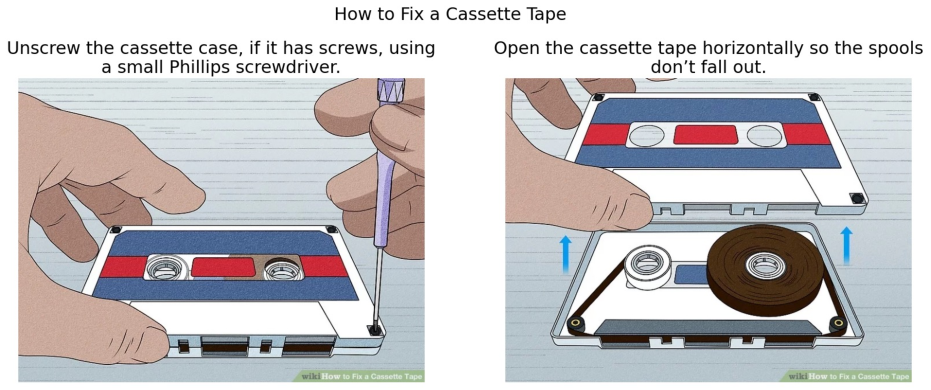
\includegraphics[width=0.45\textwidth]{figures/example_computer.pdf}}
\subfigure[Example from "Education and Communication"]{
\label{Fig.example.sub2}
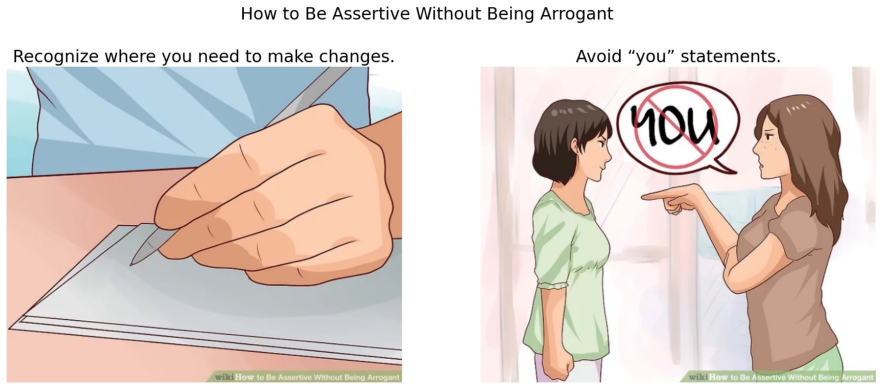
\includegraphics[width=0.45\textwidth]{figures/example_education.pdf}}
\caption{\label{fig:compare}Examples of WikiOrder dataset. Example on the left is from "Computers and Electronics" and the right one comes from "Education and Communication". We show titles, headlines and images for each pair of steps. For order prediction task, models need to predict which step comes first. The order of left example is more clear than right one.}
\end{figure*}

\subsection{Modality Gap}
Modality gap has been observed in different kinds of multimodal models\citep{xu2021videoclip,zhang2023multimodal,radford2021learning}. Liang et.al.\citep{liang2022mind} first define and analyze the phenomenon of modality gap in CLIP\citep{radford2021learning} model. The authors investigate the main causes of the modality gap and prove that simply adjusting the modality gap can change the performance of multimodal models on downstream tasks. Shi et.al.\citep{shi2023towards} conduct several experiments to prove that the loss function can directly affect the structures of different modalities in the latent space. Following previous researches, we investigate the modality gap of different models in order prediction tasks and hope to provide some insights of the influence of modality gap.

% \begin{figure*}[!htp]
% \centering
% 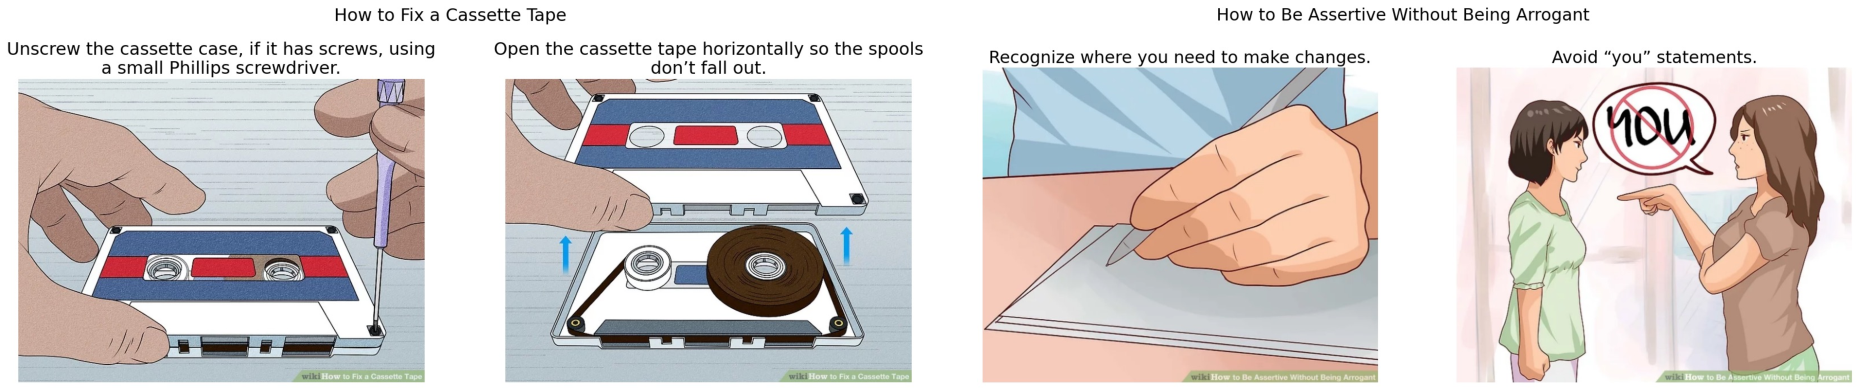
\includegraphics[scale=0.5]{figures/compare_example.pdf}
% \caption{Examples of WikiOrder dataset. Example on the left is from "Computers and Electronics" and the right one comes from "Education and Communication". We provide the titles, headlines and images for each pair of steps. For order prediction task, models need to predict which step comes first. The order of left example is more clear than right one.}
% \label{fig:compare}
% \end{figure*}


\section{WikiOrder Dataset}
Our aim is to assess current multimodal models through a novel and more challenging task. We introduce the WikiOrder dataset designed for multimodal order prediction task. We will describe the main steps of dataset construction and formulate the order prediction task in this section.

\subsection{Data Sources}
Our WikiOrder dataset comprises articles extracted from WikiHow website\footnote{https://www.wikihow.com/}. This platform hosts how-to articles covering diverse topics in daily life, including computer and information, arts and crafts, hobbies, etc. Typically, each article outlines several steps to achieve a specific goal, with each step accompanied by an illustrated picture. It's important to note that these pictures, often created by artists after reading the how-to text, may not precisely correspond to the semantic content of the step descriptions.
% WikiHow is an online wiki-style website containing various kinds of how-to articles generated by users or expertise editors. Most of the articles on the website focus on a specific topic or task. Since the goal of WikiHow is to create how-to guide for everything, the titles of articles usually start with "How to". 
WikiPlan dataset\citep{lu2023multimodal} is initially based on WikiHow articles for multimodal procedural planning tasks. The contributors of WikiPlan crawled original articles from WikiHow website and collect the task title, URL, topics, introductions and step descriptions and corresponding images. In this paper, we build upon the WikiPlan dataset to create our WikiOrder dataset.

\begin{figure*}[htp]
\centering 
\subfigure[Word cloud for verbs in titles]{
\label{Fig.wordcloud.sub1}
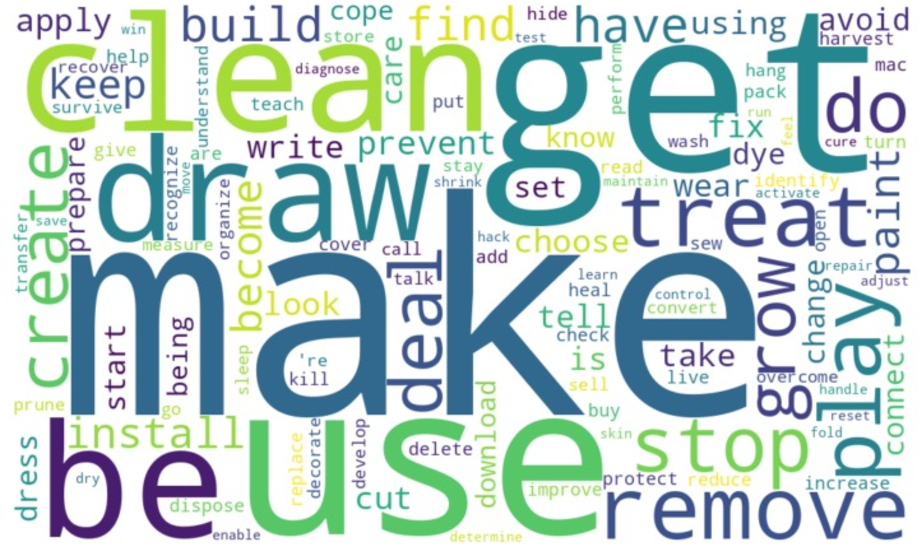
\includegraphics[width=0.45\textwidth]{figures/verb_wordcloud.pdf}}\hspace{10mm}
\subfigure[Word cloud for nouns in titles]{
\label{Fig.wordcloud.sub2}
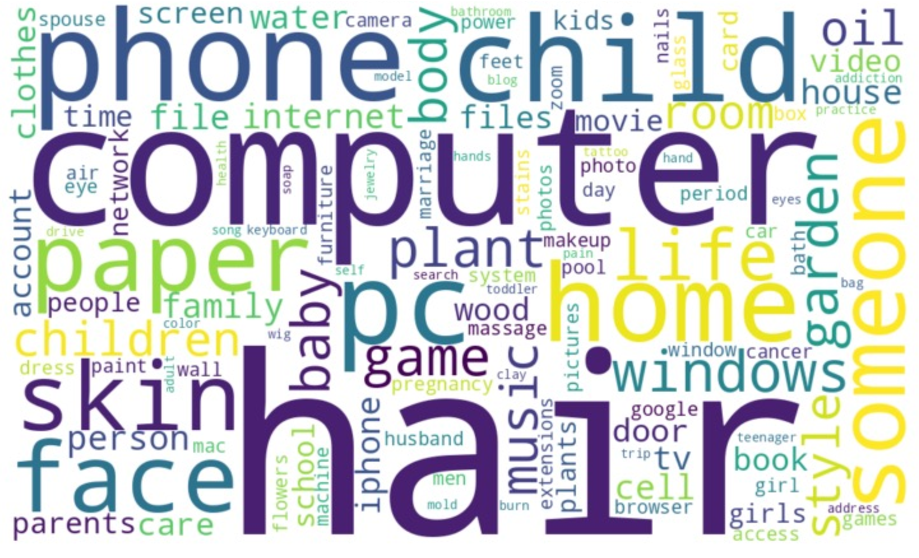
\includegraphics[width=0.45\textwidth]{figures/text_wordcloud.pdf}}
\caption{\label{fig:wordcloud}Word cloud for verbs and nouns in WikiOrder dataset. We collect all the titles and use NLTK library to extract verbs and nouns. We can find the diversity of actions and tasks.}
\end{figure*}

\subsection{Data Processing}
We take the raw WikiHow data uploaded by WikiPlan dataset contributors as the basis. The data is categorized into 10 distinct categories (see \autoref{statistics}). For each category, we first filter articles by several criteria. Firstly, to ensure each step contains information from both modalities, we filter out articles where some steps lack either images or text descriptions. Secondly, we check the shape of each image and discard articles in which the width or height of the image falls below a threshold to maintain image integrity. Then we randomly split the data of each category to three subsets: train, validation and test. 
% The proportions of these subsets are 60\%, 20\% and 20\%.

Next, we start to generate pairs by random sampling a pair of steps from articles for each subset. The number of pairs of each category is listed in \autoref{statistics}. In our settings, pairs in order (e.g. step1-step3) are assigned positive labels while those out of order (e.g. step5-step2) are assigned negative labels. For data label balance, we first retain all the sampled pairs in order and randomly invert the sequence of half of the data for each subset. This ensures an equal number of positive and negative pairs.

Each record in the WikiOrder dataset consists of five elements. “Idx” indicates the steps' source within the article. “Title” represents the original article title. “Headlines” provide concise descriptions of steps. “Label = 0” denotes pairs out of order while “Label = 1” means pairs in order. Additionally, images of corresponding steps are included in the dataset. We show two samples from two categories of our dataset in \autoref{fig:compare}.



We also illustrate the titles of all data in our dataset in \autoref{fig:wordcloud}. We use NLTK\footnote{https://www.nltk.org/} to label the collections of titles and draw word cloud plots for verbs and nouns. The result shows that our datasets contains various actions and tasks across categories.

% \MY{your case illustrations are not here. You need a subsection for data statistics}

% \begin{figure*}[!t]
% \centering
% 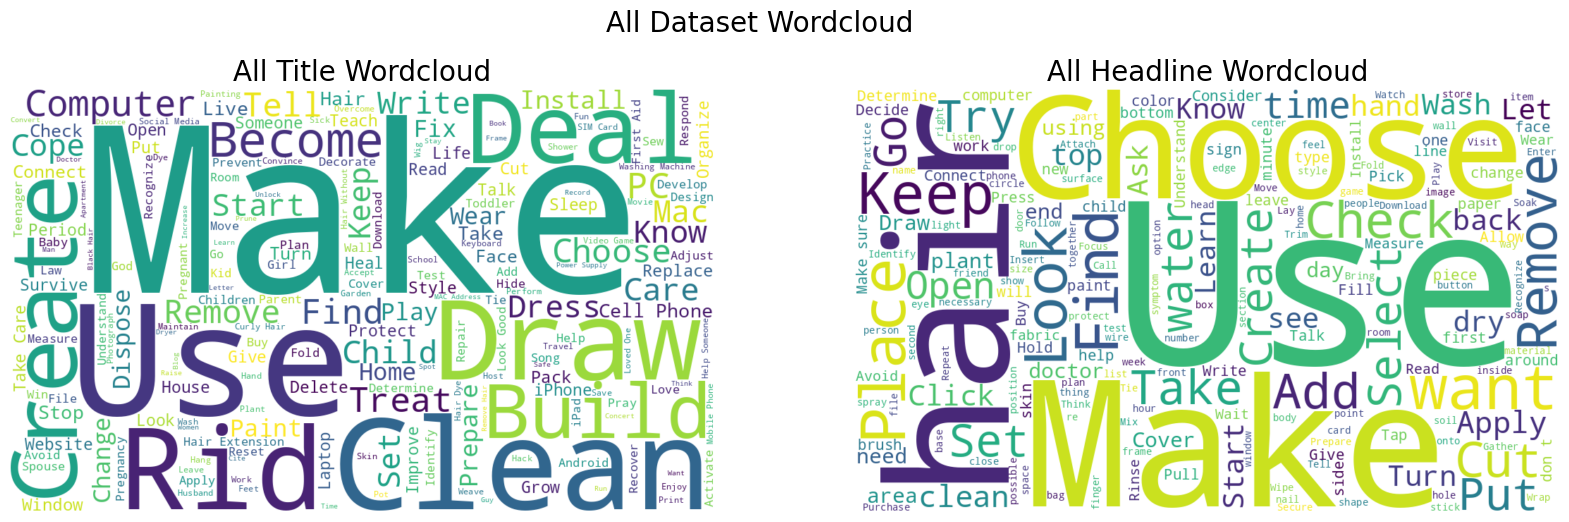
\includegraphics[scale=0.4]{figures/wikiorder_wordcloud.png}
% \caption{Word-cloud visualization of WikiOrder titles and headlines. From the title and headlines of each article, we can see the diversity of tasks.\MY{not very informative, i suggest using pos tagging first and see whether there's anything interesting in verbs, adv. nouns. etc., the purpose is to give an overview to the tasks included}}
% \label{fig:wc}
% \end{figure*}



\section{Task and Baseline Models}
WikiOrder is a multimodal dataset. We propose to use WikiOrder to evaluate the ability of different models by inferring the order of two steps. 
\subsection{Task Definition}
We formulate our order prediction task as a binary classification problem. Formally, for each data record, let the pair of headlines as $H=(h_1, h_2)$, the pair of images as $I=(i_1, i_2)$ and the title of this record as $s$, a model $M$ should predict the sequence of the pair of steps: 
\begin{equation}
    \hat{y} = M(\theta,H,I,s), ~\hat{y} \in \{0,1\}
\end{equation}

Here $\theta$ is the parameters of model $M$.

For multimodal models, both images and texts can be used. For unimodal models, they can only use either images or texts to infer the correct order.

We suppose that this task is challenging for both unimodal models and multimodal models. Unimodal models must distill crucial features from either images or texts to determine the sequential order of a step pair within a story. In contrast, multimodal models face the additional complexity of integrating knowledge from both visual and textual features to effectively tackle this task.


\subsection{Baseline Models}
In our experiments, we evaluate two multimodal models, CLIP\citep{radford2021learning} and BLIP\cite{li2022blip}. We also combine Vision Transformer (ViT)\citep{dosovitskiy2020image} and RoBERTa\citep{liu2019roberta} as another multimodal method. In order to have a fair comparison of different modalities, we take the vision encoders and text encoders from these multimodal models as unimodals, and also evaluate their performances.

\paragraph*{CLIP}
CLIP is pretrained on a large web-sourced dataset of text and images pairs. It uses contrastive learning to maximize the cosine similarity of real pairs while minimizing the cosine similarity of incorrect pairs. This approach aims to align images and texts within the same latent space. CLIP shows remarkable ability in zero-shot prediction and image-text retrieval tasks.

\paragraph*{BLIP}
Bootstrapping Language-Image Pretraining (BLIP) is a multimodal framework for unified vision-language understanding and generation. The model is jointly pretrained with three vision-language objectives: image-text contrastive learning, image-text matching, and image-text retrieval. BLIP demonstrates strong performance in various downstream multimodal tasks including image-text retrieval, image captioning, and VQA. 

\paragraph*{ViT}
Vision Transformer (ViT) is a vision model that utilizes the transformer architecture on image recognition tasks. ViT first divides the input image as a series of image patches and extract features using transformer blocks. Typically pretrained on extensive datasets like ImageNet, ViT can be applied to various vision tasks by modifying its architecture.

\paragraph*{RoBERTa}
RoBERTa is a variant of the BERT\citep{devlin2018bert} model. Compared with BERT, RoBERTa is pretrained on a much larger dataset and applies more delicate training strategies. Additional data and more extensive pre-training make RoBERTa outperform BERT and other language models on many NLP tasks.



\begin{table*}[!tp]
\centering
\caption{Experimental results on 10 categories of WikiOrder datset. We evaluate 3 baseline models: CLIP, ViT+RoBERTa and BLIP with data in three kinds of modalities. The reported results are the average scores of accuracy. For modalities, \textbf{V+T}=Vision+Text, \textbf{V}=Vision-only and \textbf{T}=Text-only. For categories, \textbf{HC}.=Hobbies and Crafts, \textbf{AE.}=Arts and Entertainment, \textbf{CE.}=Computers and Electronics, \textbf{EC.}=Education and Communication, \textbf{FL.}=Family Life, \textbf{HG.}=Home and Garden, \textbf{PS.}=Personal Care and Style, \textbf{PR.}=Philosophy and Religion.}
\label{results}
\begin{tabular}{lccccccccc}
\hline
\multirow{2}{*}{Category} & \multicolumn{3}{c}{CLIP} & \multicolumn{3}{c}{ViT+RoBERTa} & \multicolumn{3}{c}{BLIP} \\ \cline{2-10} 
 & \multicolumn{1}{c}{V+T} & \multicolumn{1}{c}{V} & \multicolumn{1}{c}{T} & \multicolumn{1}{c}{V+T} & \multicolumn{1}{c}{V} & \multicolumn{1}{c}{T} & \multicolumn{1}{c}{V+T} & \multicolumn{1}{c}{V} & \multicolumn{1}{c}{T} \\ \hline
AE. & 0.599 & 0.622 & 0.593 & 0.701 & 0.684 & 0.637 & 0.732 & 0.699 & 0.603 \\
CE. & 0.677 & 0.664 & 0.669 & 0.759 & 0.716 & 0.690 & 0.817 & 0.789 & 0.675 \\
EC. & 0.539 & 0.549 & 0.541 & 0.629 & 0.613 & 0.580 & 0.665 & 0.696 & 0.518 \\
FL. & 0.538 & 0.665 & 0.538 & 0.703 & 0.657 & 0.532 & 0.695 & 0.721 & 0.564 \\
Health & 0.561 & 0.708 & 0.560 & 0.733 & 0.723 & 0.600 & 0.738 & 0.709 & 0.586 \\
HC. & 0.663 & 0.704 & 0.658 & 0.773 & 0.733 & 0.702 & 0.780 & 0.786 & 0.679 \\
HG. & 0.628 & 0.601 & 0.622 & 0.730 & 0.692 & 0.651 & 0.734 & 0.717 & 0.643 \\
PS. & 0.612 & 0.693 & 0.615 & 0.728 & 0.707 & 0.561 & 0.788 & 0.746 & 0.627 \\
PR. & 0.580 & 0.586 & 0.590 & 0.696 & 0.674 & 0.615 & 0.715 & 0.701 & 0.615 \\
Travel & 0.597 & 0.577 & 0.580 & 0.644 & 0.589 & 0.558 & 0.743 & 0.741 & 0.585 \\ \hline
\end{tabular}
\end{table*}

\subsection{Training and Testing}
Given the substantial disparity between the order prediction task and models' pretraining tasks, it's necessary to fine-tune the models on WikiOrder training set. Similar to linear probe experiments of CLIP, we extract features by encoders and apply a linear head on the features for classification. All the parameters are trainable for fine-tuning. Take multimodal models as an example. For each kind of data $H=(h_1,h_2), s$ and $I=(i_1,i_2)$, we first use vision encoder $V(\theta_v)$ and text encoder $T(\theta_t)$ to extract features:
\begin{equation}
\begin{split}
    t &= T(\theta_t,[s;H])\\
    v &= V(\theta_v,I)
\end{split}
\end{equation}

Here $[;]$ means concatenation operation. $t$ and $v$ are text embedding and image embedding. We combine the title with the input text to provide more information about the story to the model.

Then we concatenate the features and put forward to the classification head:

\begin{equation}
\begin{split}    
    l &= W*[t;v]+b, l\in \mathbb{R}^2 \\
    \hat{y} &= \arg \max (l)
\end{split}
\end{equation}

 $W$ and $b$ are layer weight matrix and bias. The final prediction is the position of output feature with higher probability.

For unimodal models, the features are extracted by corresponding encoders. For vision models we use $I$ and $s$ while for text models we use $H$ and $s$. It's important to specify that for vision models, the text encoder of their paired counterpart (e.g., for ViT in the CLIP model, the paired text encoder is the text transformer) is employed to encode the title $s$, and concatenate the text embedding the image embedding. We emphasize that the title of each data record serves as the context for all models, ensuring that vision, text, and combined vision+text models leverage information from the title. And still, the vision model exclusively use images of the steps when training and testing. When testing, we maintain the same architecture and evaluate the fine-tuned models on the WikiOrder test set. 

\section{Experiment}

\subsection{Experimental Setup}
We fine-tuned CLIP, BLIP and ViT+RoBERTa with training dataset in three kinds of modalities. All the models are initialized with pretrained weights from HuggingFace website\footnote{https://www.huggingface.co/}. We use "clip-vit-base" (151.28M), "blip-itm-base" (223.74M) and "vit-base"+"roberta-base" (211.04M) in our experiments\footnote{The number of parameters in the parenthesis is for multimodal model and contains the classification head.}. We fine-tuned these models on 1 Nvidia GeForce RTX 3090 card. We use the Adam\citep{kingma2014adam} optimizer with learning rate $10^{-5}$, batch size of 4 and run 5 epochs. The model for testing is selected by the highest accuracy on the validation set.
% \MY{Add a subsection for metrics. }

\subsection{Evaluation Metrics}
We choose accuracy as the metric to assess the performance of different models. Accuracy is computed as the ratio of correctly predicted orders to the total number of test data for each category::

\begin{equation}
    Acc_i = \frac{\text{Number of Correct Predictions in } i}{\text{Total Number of Predictions in }i}    
\end{equation}

Here $i$ indicates the category name.


\subsection{Main Results}

\begin{figure*}[ht]
\centering 
\subfigure[Computers and Electronics]{
\label{Fig.mg.sub1}
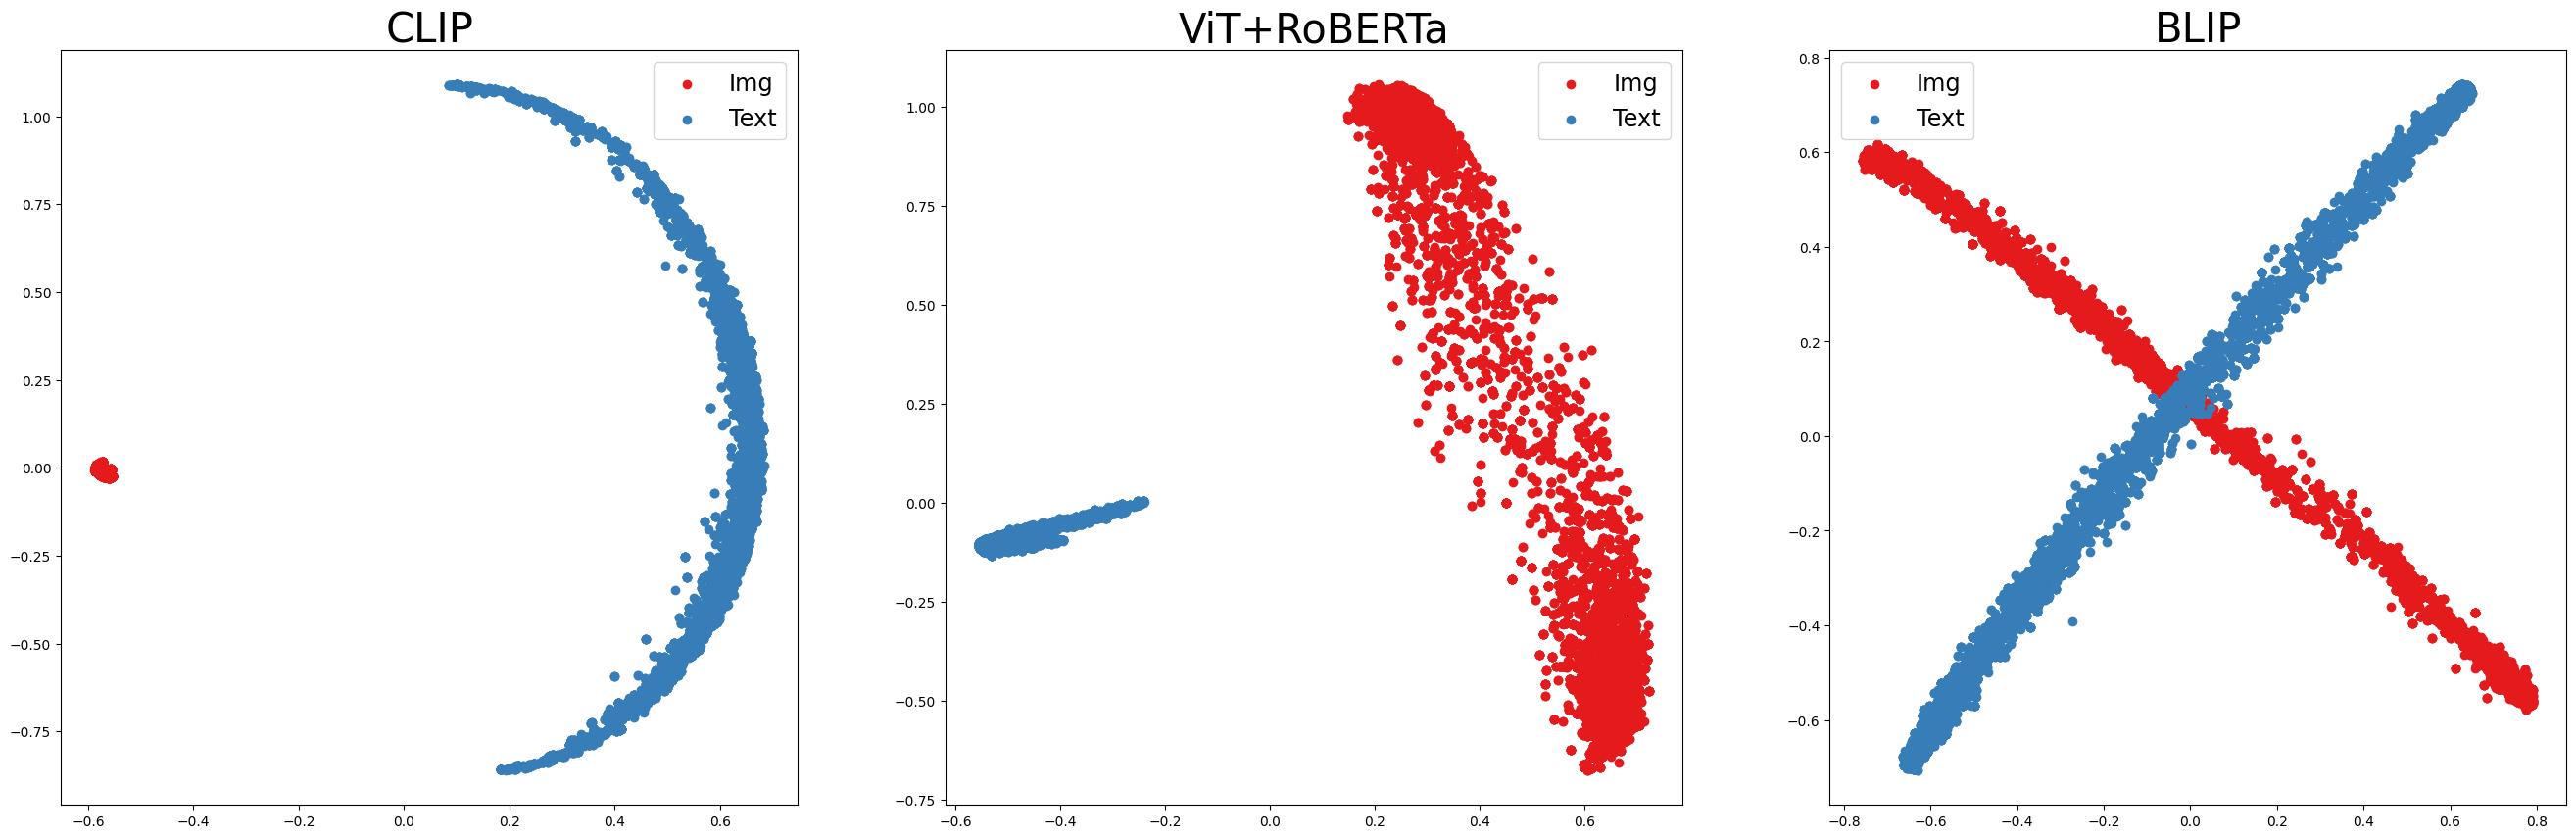
\includegraphics[width=1.0\textwidth]{figures/mg_computer.png}}\hspace{10mm}
\subfigure[Education and Communication]{
\label{Fig.mg.sub2}
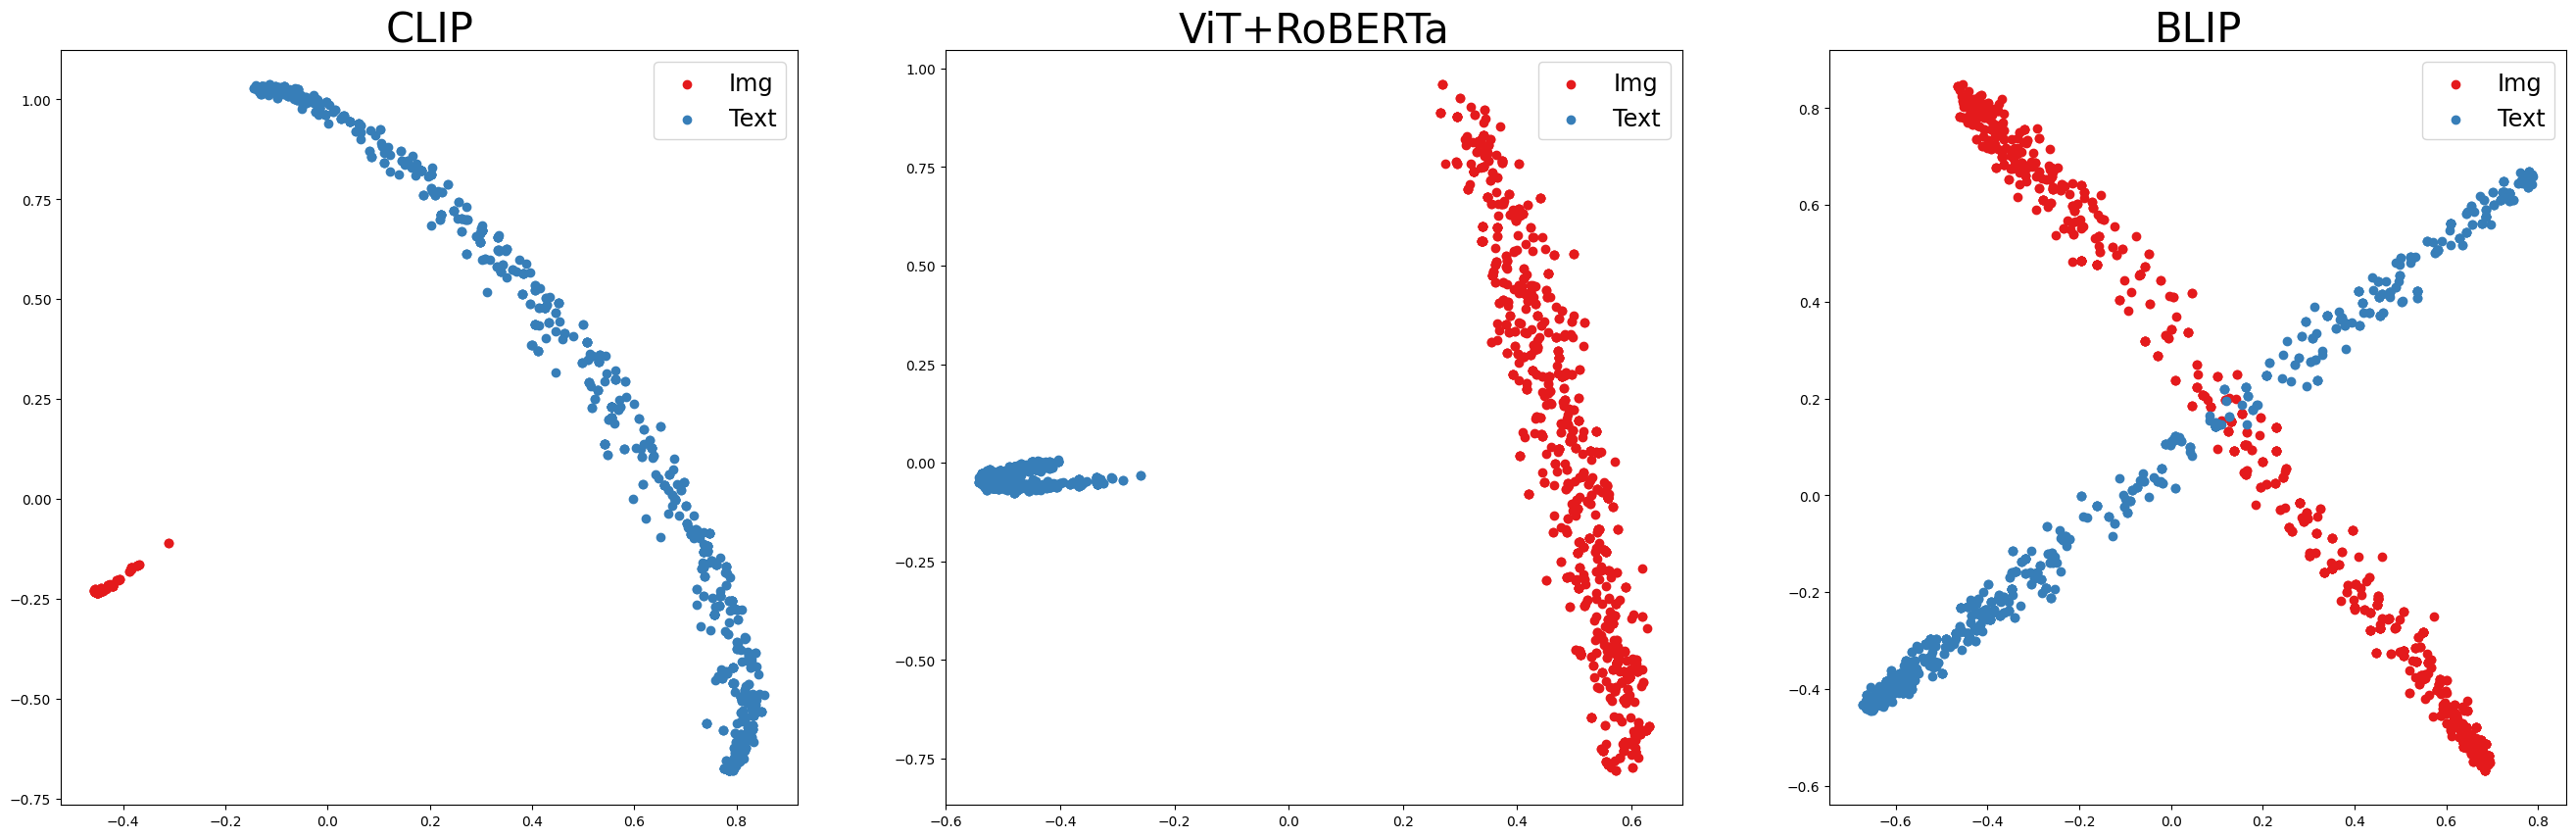
\includegraphics[width=1.0\textwidth]{figures/mg_education.png}}
\caption{\label{fig:mg}Illustration of modality gap in vision-text models. We show the modality gap in "Computers and Electronics" (in Subplot a) and "Education and Communication" (in Subplot b). For illustration, image features and text features are transformed to 2D features using PCA method. Red dots are image embeddings while blue ones are text embeddings.}
\end{figure*}

% \begin{figure*}[!t]
% \centering
% 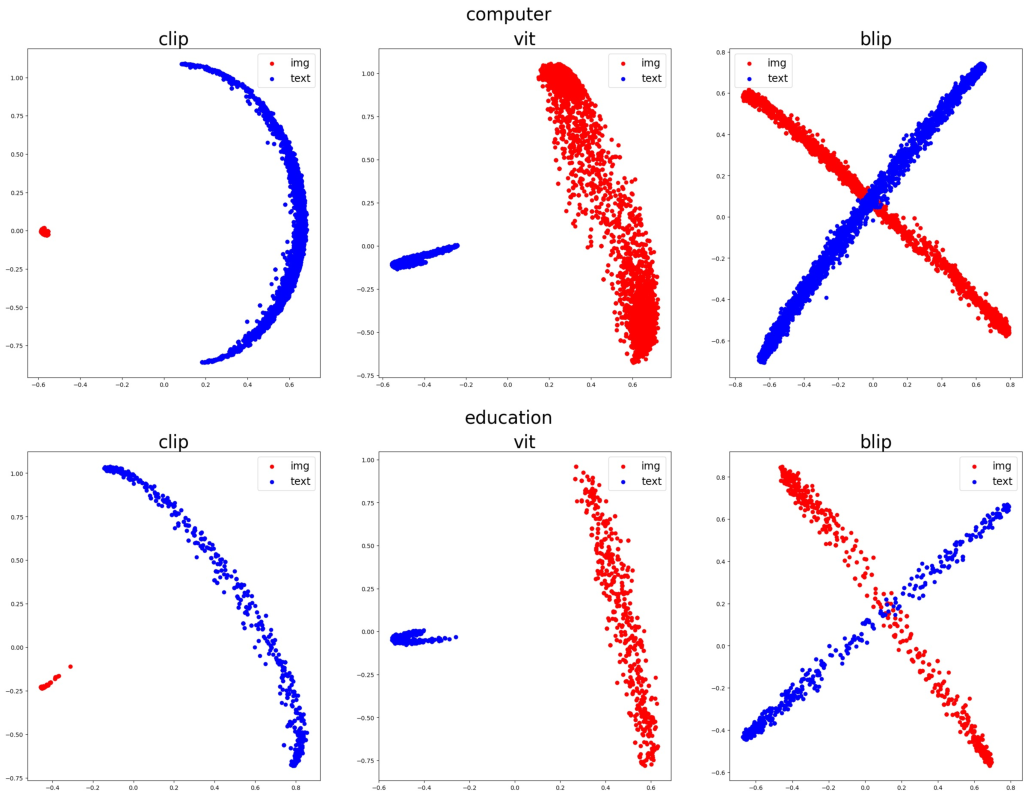
\includegraphics[scale=0.9]{figures/mg.pdf}
% % \includegraphics[scale=0.8]{mixer2.pdf}
% \caption{Illustration of modality gap in vision-text models. We show the modality gap in "Computers and Electronics" and "Education and Communication". For illustration, image features and text features are transformed to 2D features using PCA method.}
% \label{fig:mg}
% \end{figure*}


\autoref{results} presents the evaluation outcomes of different models in the order prediction task. Here we report the average accuracy scores for each categories and each model.

Comparing three modalities, for ViT+RoBERTa and BLIP, vision+text models consistently outperform both vision-only and text-only models across most categories. This finding is consistent with prior research that multimodal models exhibit superior performance in reasoning tasks. The assumption is that multimodal models can leverage both image features and text features during prediction, even with a simple concatenation of features. Notably, vision-only models outperform text-only models in all categories. Besides, the results of vision+text models closely resemble those of vision-only models, rather than text-only models. This suggests that image features carry a higher weight and contribute to better performance compared to text features. We suggest the reason is that in WikiOrder, images are illustrations of texts and potentially convey richer information than texts alone.

The results of CLIP is significantly different from ViT+RoBERTa and BLIP. Vision-only models generally achieve best results among three modalities. The gap between vision-text performance and text-only performance is smaller than the other two models. We attribute this deviation in CLIP's performance to the misalignment between pretraining tasks and the order prediction task. CLIP is pretrained in contrastive learning method and the embeddings of images and texts are expected to be aligned in one latent space. However, in WikiHow dataset, images and texts lack this alignment. Even with fine-tuning on the training set, CLIP struggles to adapt to the new task and new dataset. On the other hand, BLIP shows highest performance among three models. This may attributed to the diverse pretraining task of BLIP. Therefore, compared with CLIP, BLIP benefits from various pretraining tasks and can better adapt to WikiHow data and order prediction task.

Model performances also exhibit variability across categories. Take BLIP vision+text model as an example, the highest accuracy is observed in "Computers and Electronics" while the lowest is in "Education and Communication". The performances of CLIP, ViT+RoBERTa and BLIP among different categories are consistent, thus we can label the categories as "difficult category" or "easy category" by the evaluation results. Category difficulty is influenced by two factors. First of all, categories with less stories tend to be more difficult, as the scarcity of data heightens the difficulty for models to discern patterns. On the other hand, the sequential relationships between steps vary in categories. Stories in easy categories are more orderly than those in difficult ones. Consequently, models are more likely to infer the sequential relationship in easy categories. Besiedes, across all categories, the best performance is around 0.7, which is not a high score for binary classification tasks. We believe that this finding can also prove the difficulty of the order prediction task.


% \begin{figure*}[!tp]
% \centering
% 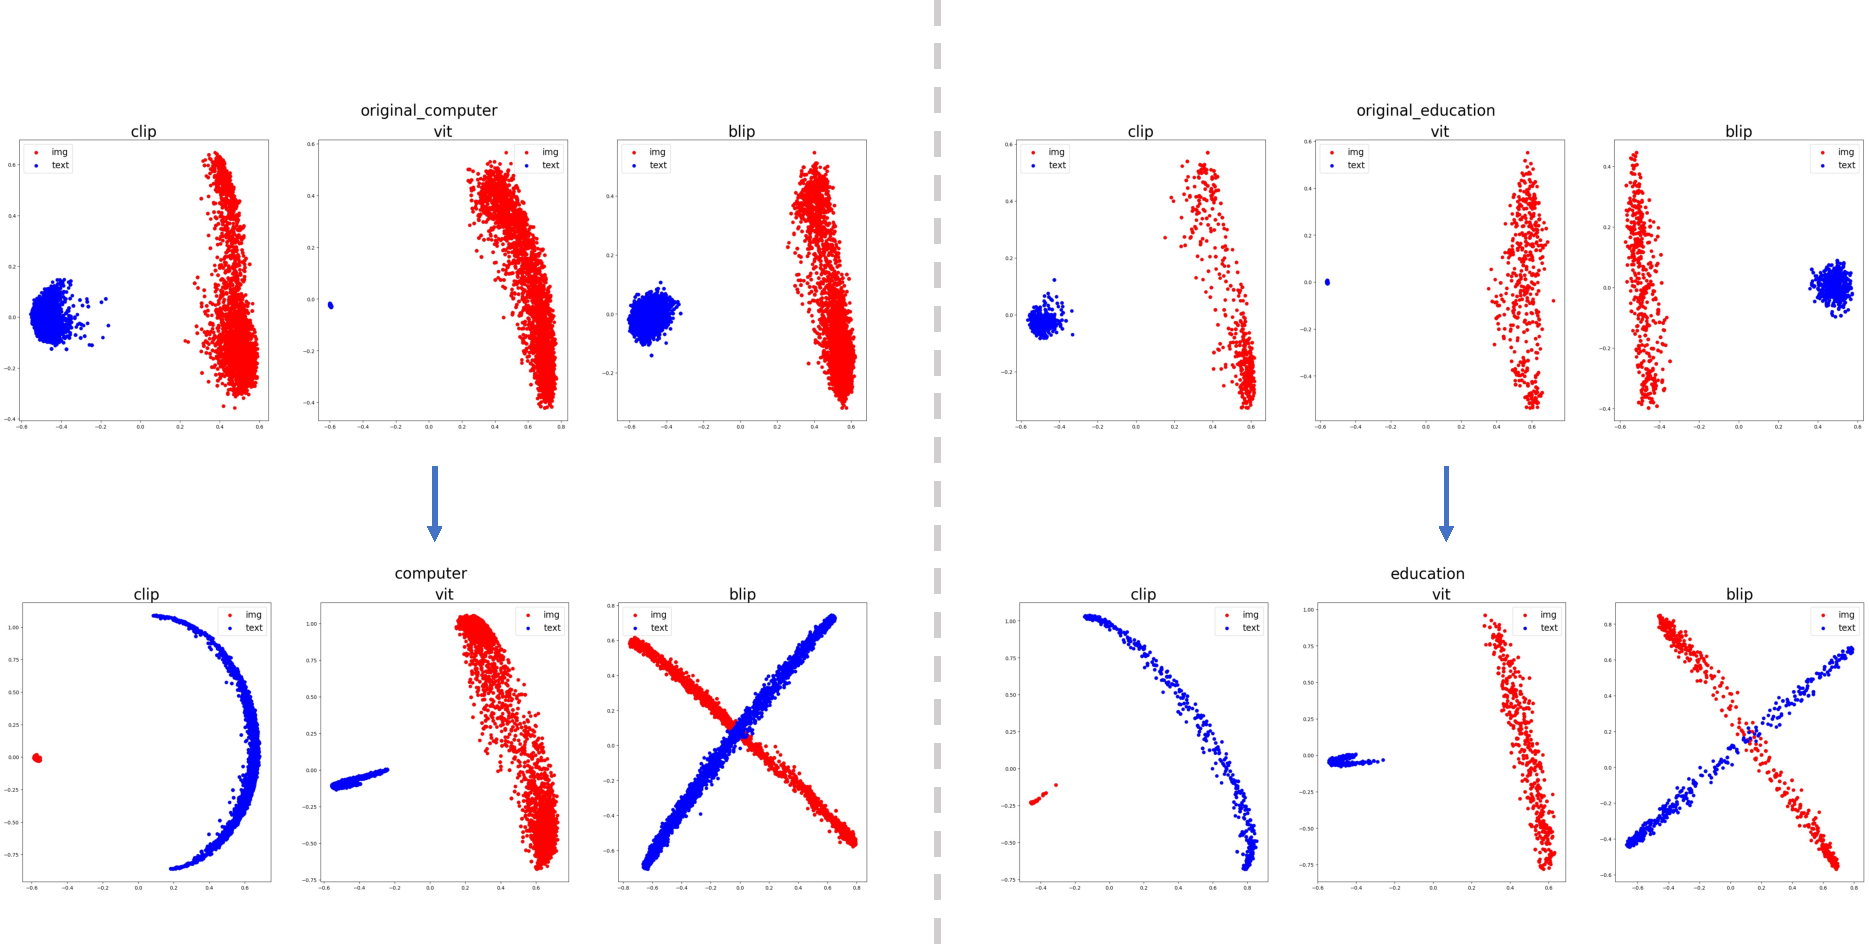
\includegraphics[scale=0.5]{figures/mg_change.pdf}
% % \includegraphics[scale=0.8]{mixer2.pdf}
% \caption{Illustration of modality gap change before and after fine-tuning in vision-text models. We show the change in "Computers and Electronics" and "Education and Communication". Figures in the upper row are from pretrained models while figures below are the results of fine-tuned models in different categories.}
% \label{fig:mg-change}
% \end{figure*}


\begin{figure*}[htbp]
    \centering
    \subfigure{
        \rotatebox{90}{\scriptsize{~~~~~~~~~~~~~Pretrained}}
        \begin{minipage}[t]{0.45\linewidth}
            \centering
            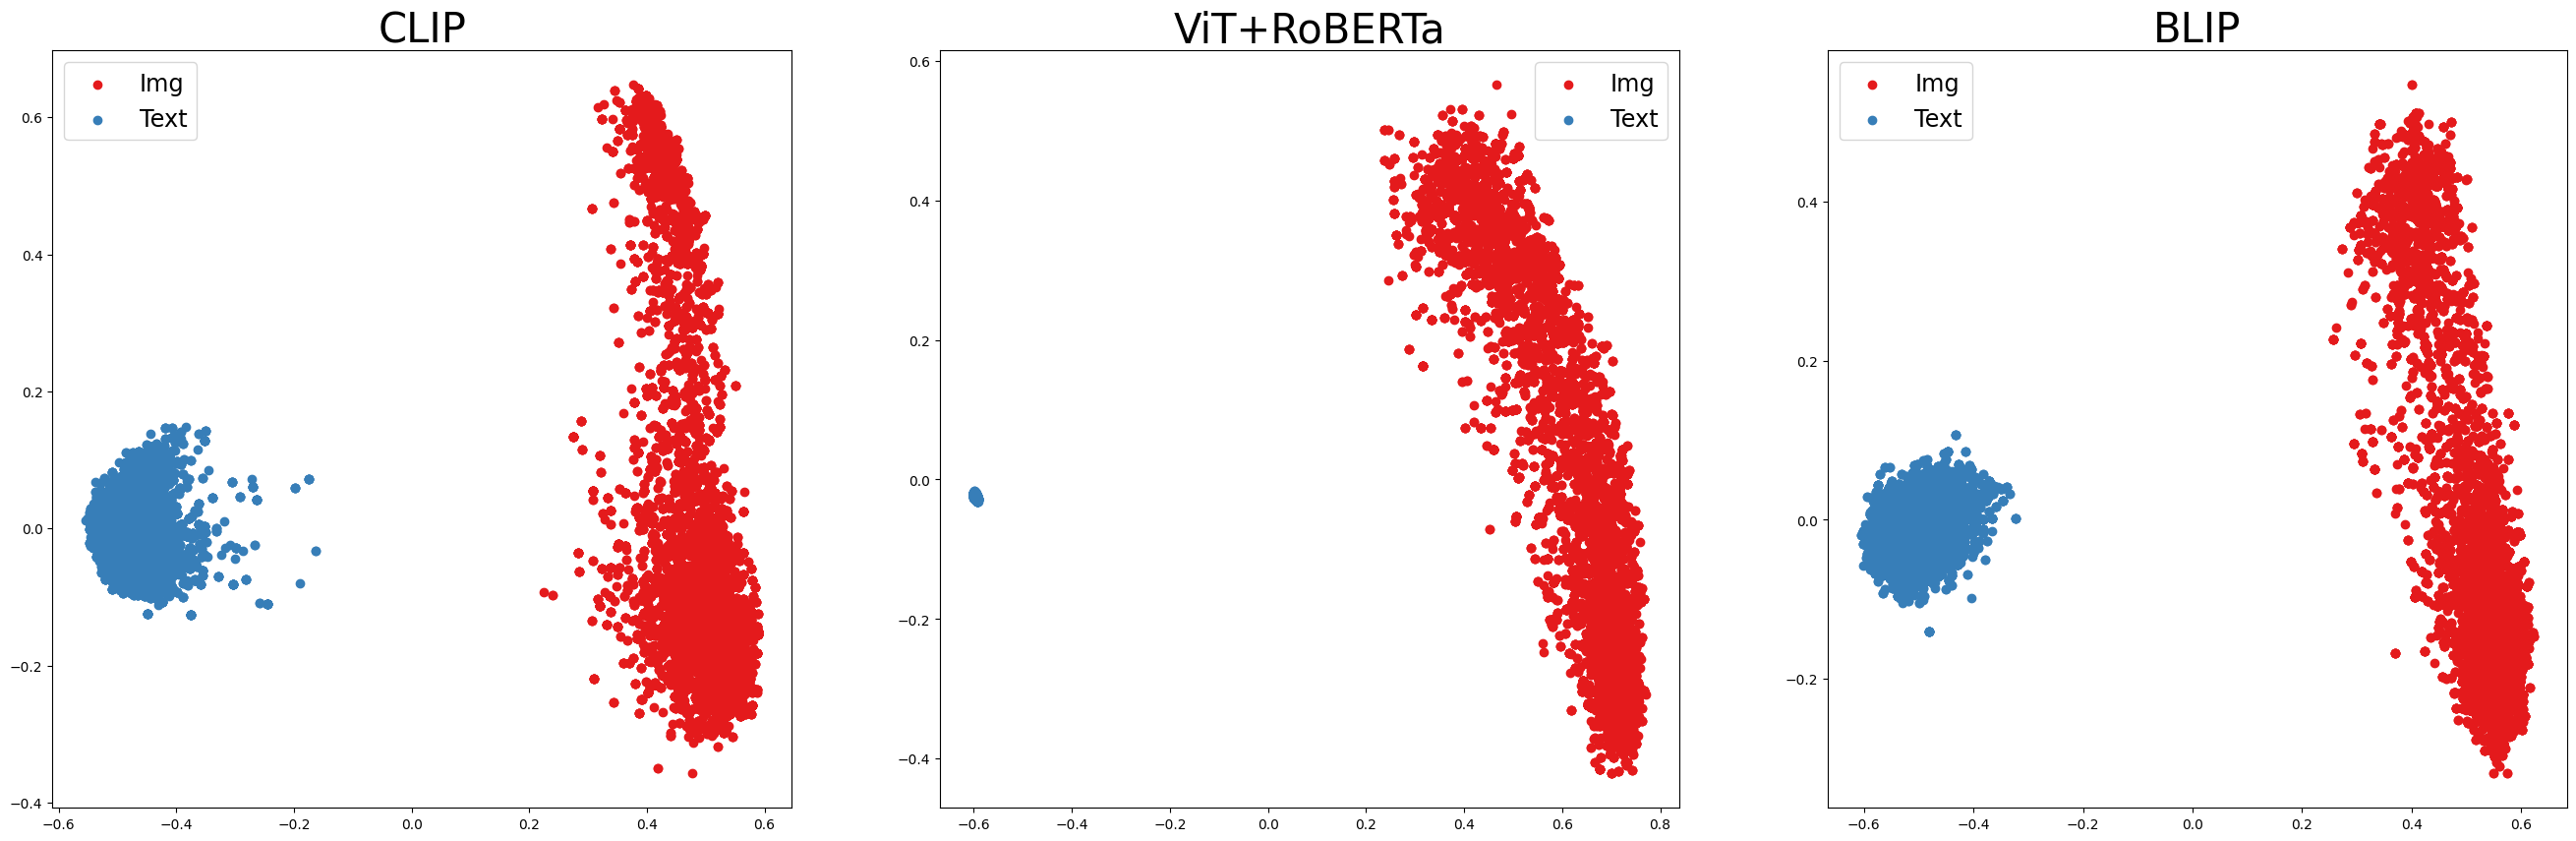
\includegraphics[width=1\linewidth]{figures/ori_computer.png}
        \end{minipage}
    }\hspace{5mm}
    \subfigure{
        \begin{minipage}[t]{0.45\linewidth}
            \centering
            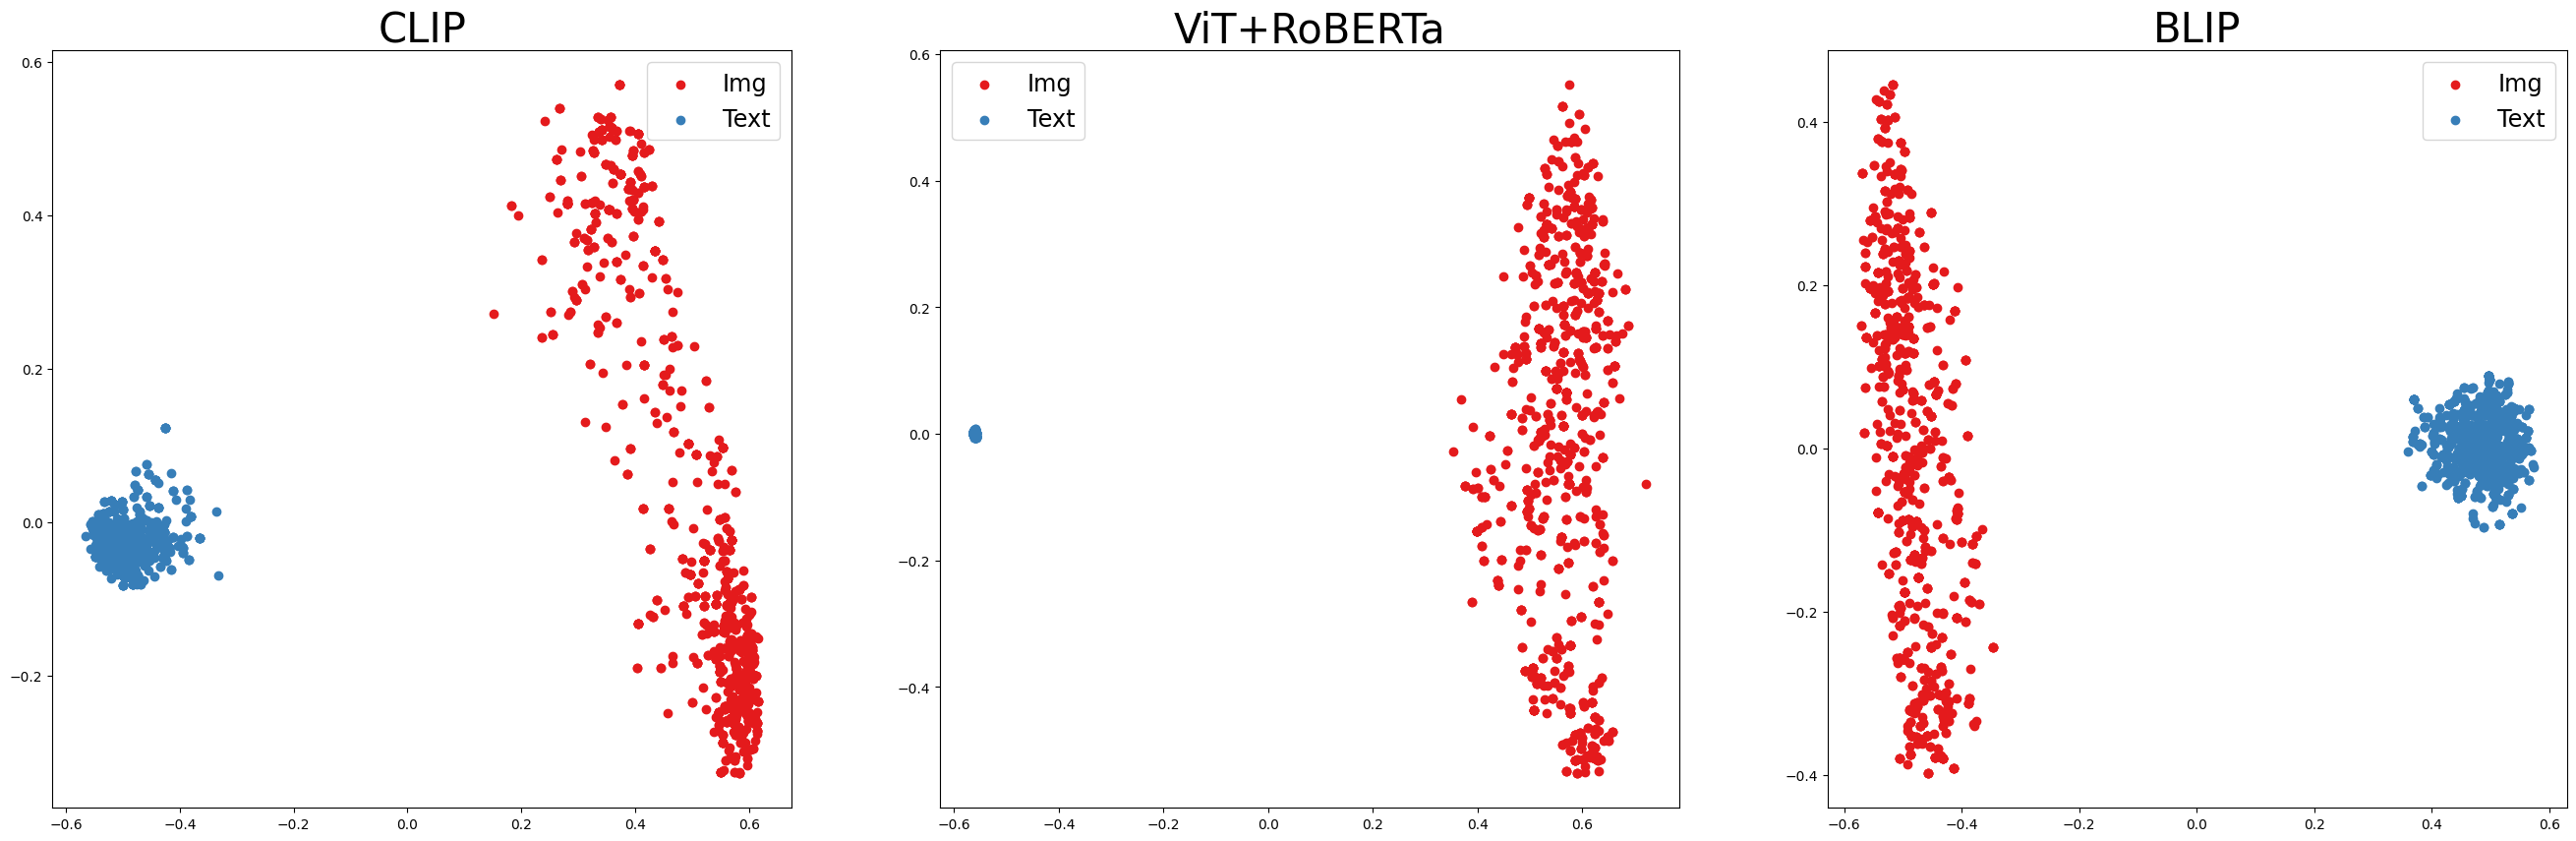
\includegraphics[width=1\linewidth]{figures/ori_education.png}
        \end{minipage}
    }
    \setcounter{subfigure}{0}
    
        \subfigure[Computers and Electronics]{
        \rotatebox{90}{\scriptsize{~~~~~~~~~~~~~Fine-tuned}}
        \begin{minipage}[t]{0.45\linewidth}
            \centering
            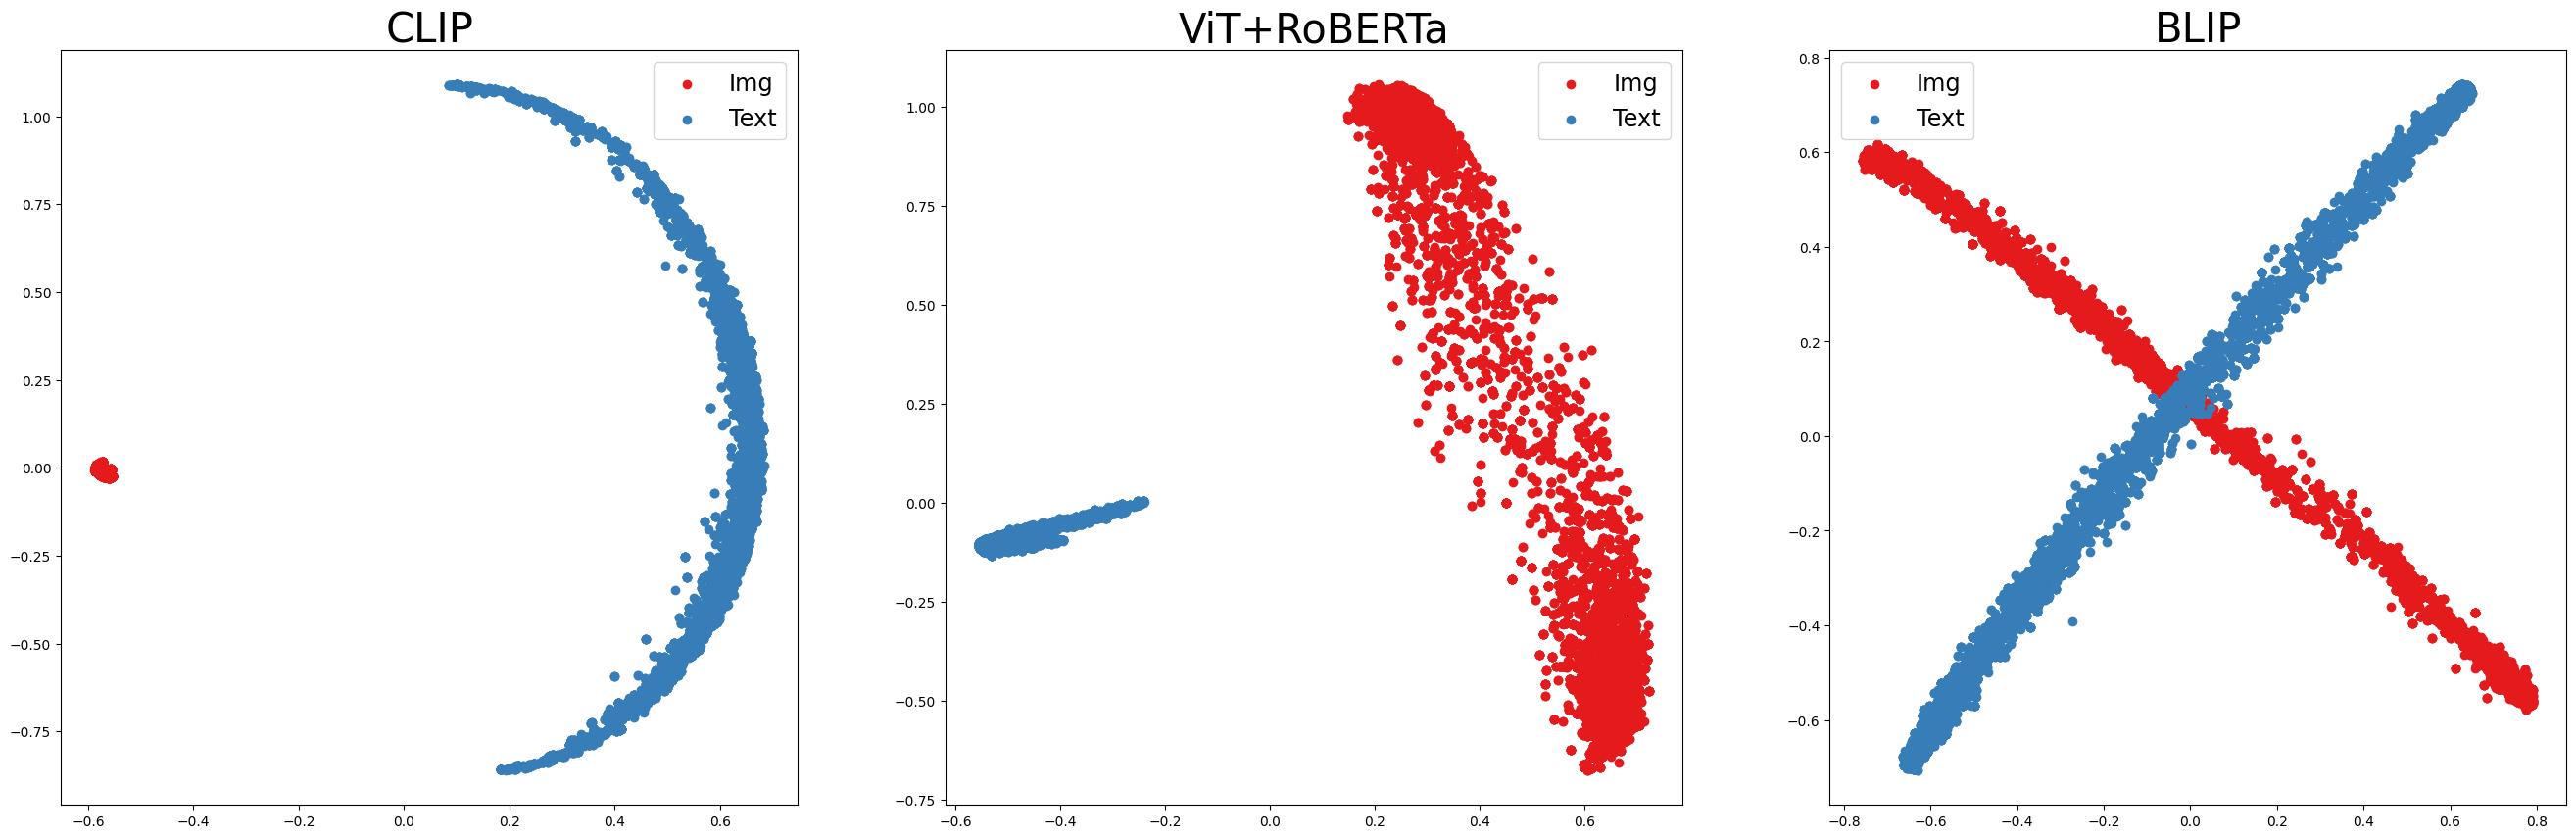
\includegraphics[width=1\linewidth]{figures/mg_computer.png}
        \end{minipage}
    }\hspace{5mm}
    \subfigure[Education and Communication]{
        \begin{minipage}[t]{0.45\linewidth}
            \centering
            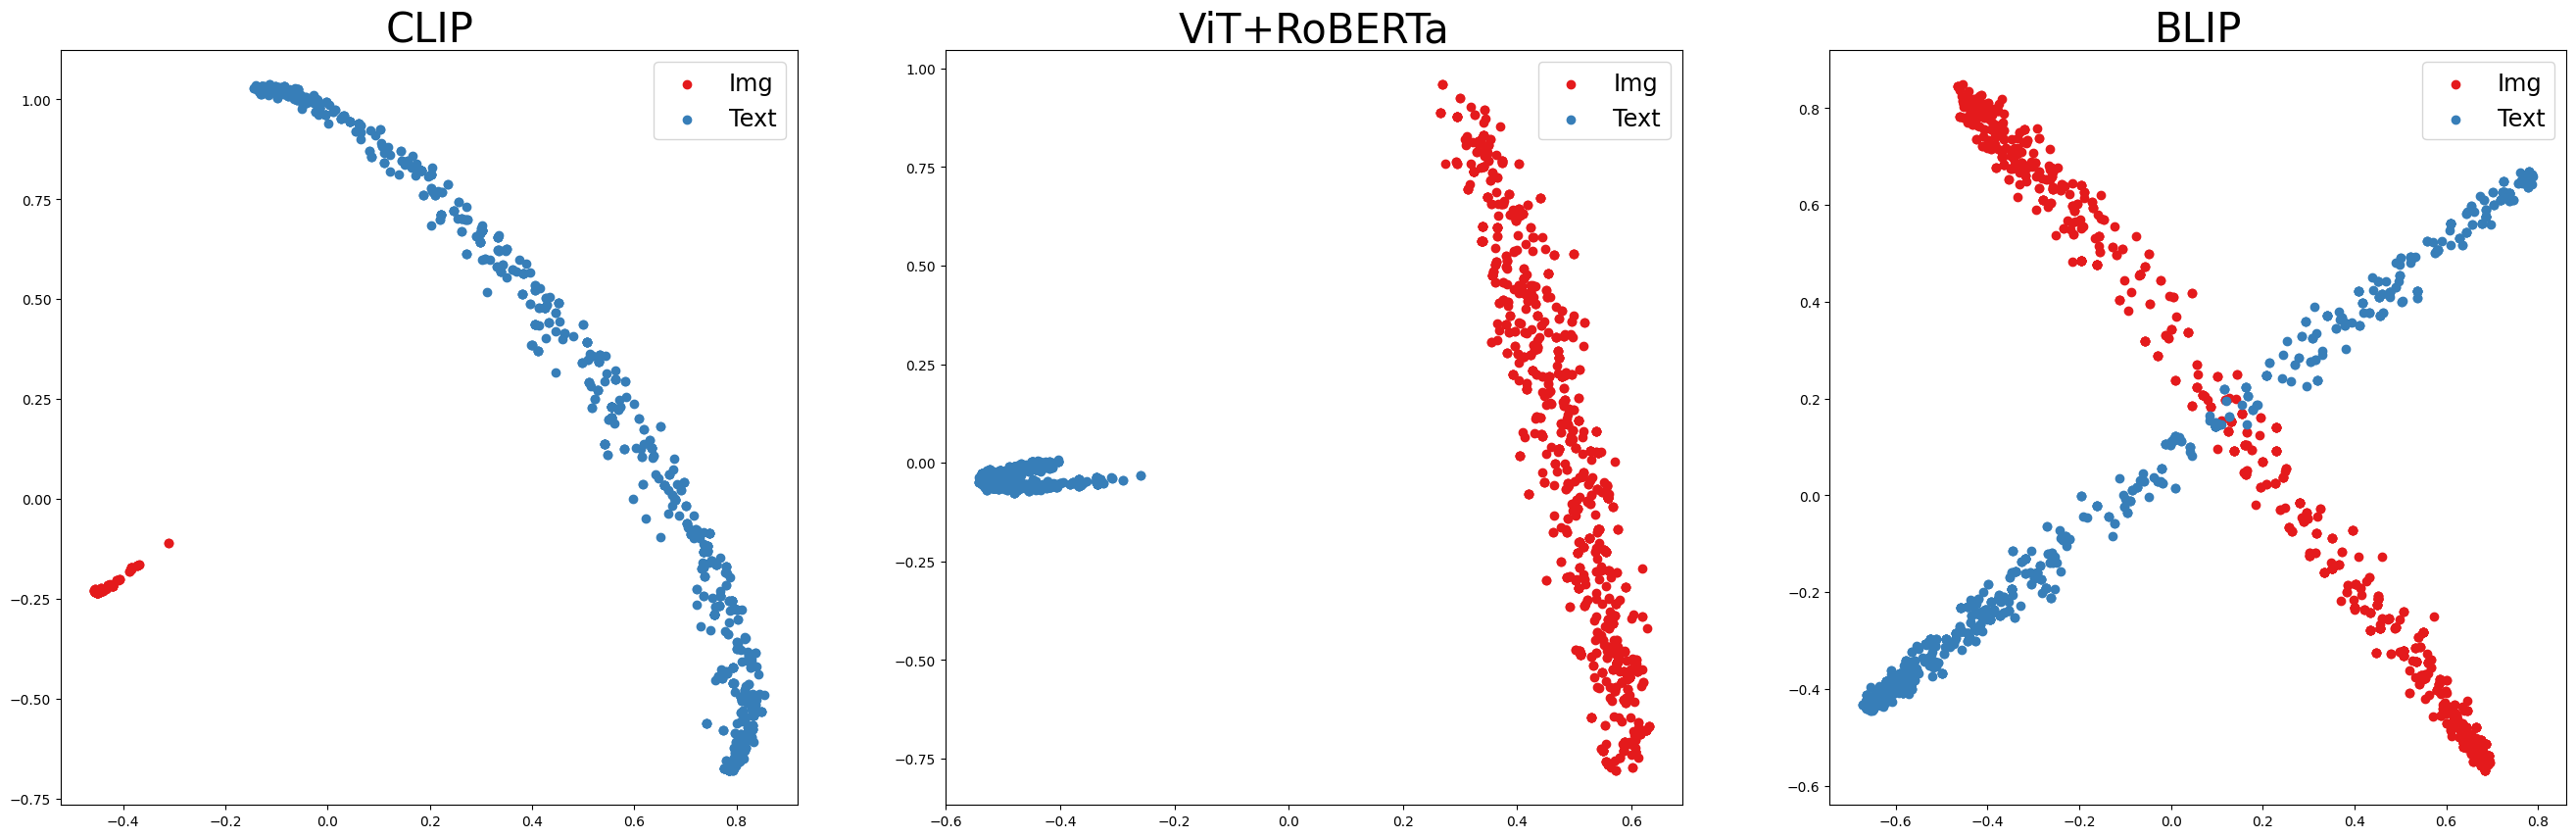
\includegraphics[width=1\linewidth]{figures/mg_education.png}
        \end{minipage}
    }
    \caption{\label{fig:mg-change}Illustration of modality gap before and after fine-tuning in vision-text models. We show the change in "Computers and Electronics" and "Education and Communication". Figures in the upper row are from pretrained models while figures below are the results of fine-tuned models in different categories.}
\end{figure*}


\subsection{Modality Gap}

Modality gap refers to the phenomenon where the image embeddings and text embeddings are located in two completely separate regions of the embedding space \citep{liang2022mind}. Formally, modality gap between vision and text can be defined as the distance between the center of image embeddings and text embeddings: 

\begin{equation}
    gap=\left \lVert \frac{1}{n}\sum_{i=1}^n x_i - \frac{1}{n}\sum_{i=1}^n y_i \right \rVert
\end{equation}

Here $x_i$ and $y_i$ are the normalized embeddings of image features and text features of the dataset.

Here we employ the concept of modality gap to explain the performance gap of three baseline models. Following the paper mentioned above, we use Principal Component Analysis (PCA) tool of Scikit-Learn package to visualize the modality gap in three multimodal models. In \autoref{fig:mg}, we show the data distributions of two categories: "Computers and Electronics" and "Education and Communication". These two categories are considered as the easiest one and the most difficult one. We first extract image embeddings and text embeddings by image encoder and text encoder from fine-tuned model. Then we apply L2 normalization on each embedding and reduce the dimension to two dimensions by PCA tool. Next, we plot the distribution of image embeddings (in red) and text embeddings (in blue) of each model. 

Our visualization results align with previous research, showing that visual features and textual features tend to clulster. We think the clustering of embeddings intensifies the difficulty for models to deal with order prediction task, especially when the embeddings for all images are similar. In addition, we have some interesting findings in our experiments. For CLIP, the distribution of visual features are more clustered than other models and the modality gap is also larger. Based on these results, we suggest that the modality gap of CLIP lead to the poor performance of CLIP in vision+text tasks. In contrast, both ViT+RoBERTa and BLIP exhibit more dispersed embeddings, leading to superior results for vision+text tasks compared to CLIP. Additionally, we find that the distributions of image embeddings and text embeddings of BLIP intersect at the center and the modality gap is the smallest among three models. This observation provides insight into why BLIP attains the highest score in vision+text tasks.

Furthermore, in order to investigate how these models adapt to the order prediction task, we compare the modality gap between pretrained models ("original models") and corresponding models fine-tuned in WikiOrder dataset ("fine-tuned models"). As depicted in \autoref{fig:mg-change}, we can find an obvious transition from original models to fine-tuned models. First of all, for original models, text embeddings tend to be closer to image embeddings. This can show the variance of images is larger than texts. For Vit+RoBERTa, where the vision model and text model of this pair are pretrained separately, the alignment of these two modalities are not well. Secondly, considering the fine-tuned models, distributions of text embeddings change a lot, especially for CLIP. Text embeddings become more desperate while the image embeddings are more clustered. For BLIP model, both vision and text embeddings experience considerable changes, with improved alignment between these modalities in fine-tuned models compared to original ones. This transition of embeddings underscores the existence of a gap between our order prediction task and pretrained tasks (e.g. image-text matching). Consequently, our dataset provide a novel perspective for evaluating the performance of multimodal models.

\section{Analysis}

\begin{figure*}[!tp]
\centering 
\subfigure[Image matters]{
\label{Fig.case.sub1}
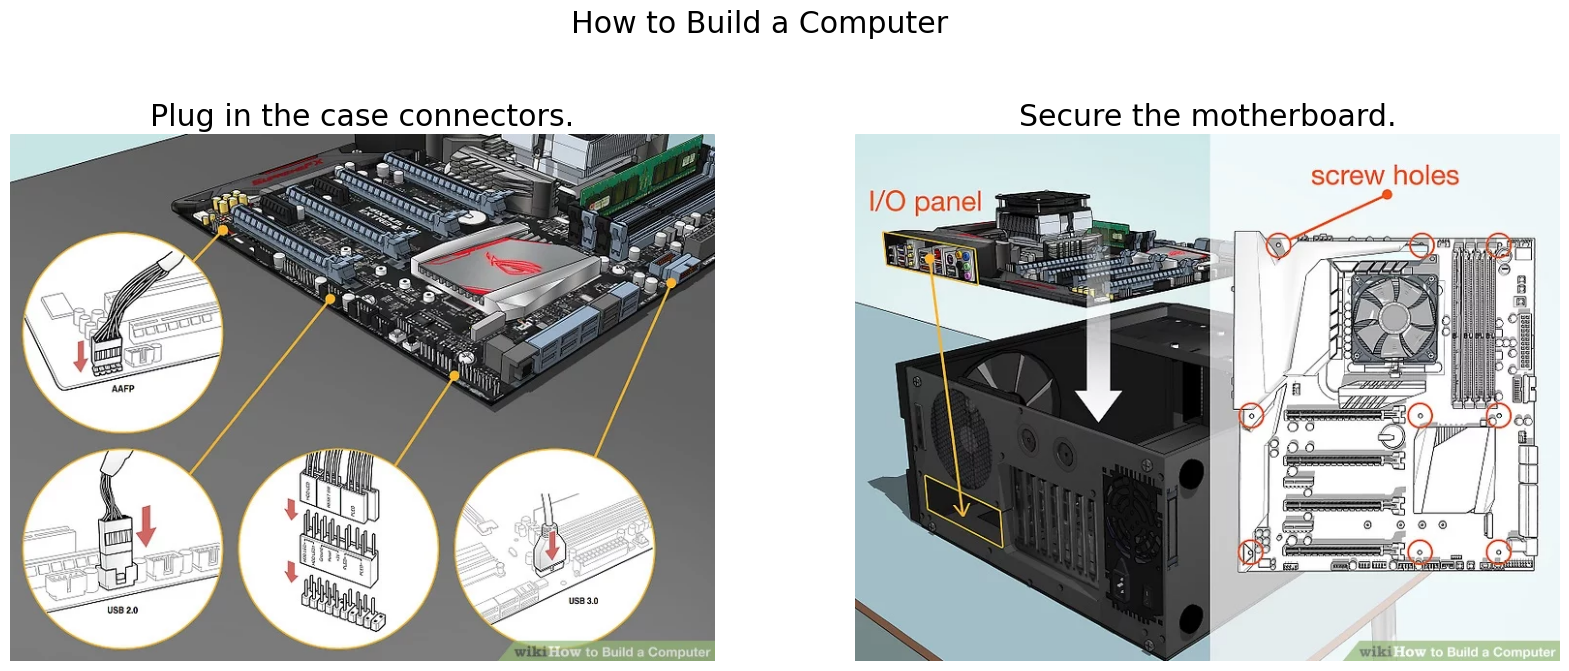
\includegraphics[width=0.45\textwidth]{figures/case_img_better.png}}\hspace{10mm}
\subfigure[Text matters]{
\label{Fig.case.sub2}

\includegraphics[width=0.45\textwidth]{figures/case_text_better.png}}
\caption{\label{fig:case}Case study of modality importance. Here we show two examples from "Computers and Electronics" category. In Subplot a, the image is more import in order prediction while in Subplot b, the text matters.}
\end{figure*}

Here we show some cases to compare the effect of different modalities in order prediction task (See \autoref{fig:case}). For Sub-figure a, text descriptions are ambiguous due to the undefined context of "case connectors". However, if we inspect the images, placing the motherboard should precede plugging in the connectors on the motherboard. Subseqently, in Sub-figure b, the images are similar, making it challenging to determine the order based solely on visual cues. However if we investigate the texts, writing down things should precede giving the message to the person. This scenario exemplifies a significant challenge for models in predicting order on the WikiOrder dataset, as it necessitates the fusion of information from both modalities to derive accurate predictions.

% \MY{You should definitely include case analysis here, on what cases vision is more helpful and where text is. Also those vision+text, show your readers that this is interesting and even challenging for humans.}

\section{Conclusion}
In this paper, we introduce WikiOrder, a multimodal dataset. WikiOrder is extracted from WikiHow website which contains instruction articles for daily tasks in various categories. Compared with other multimodal datasets for image captioning and image-text retrieval tasks, WikiOrder presents a unique challenge as the alignment between images and texts is less obvious. For the first time, we propose a multimodal order prediction task to evaluate the reasoning ability of diverse multimodal models.

Experiments of three multimodal models on WikiOrder dataset show the difference between order prediction task and pretrained tasks. We find that ViT+RoBERTa and BLIP exhibit better adaptation to order prediction task compared to CLIP. We also find significant differences of performance across modalities. These results are elucidated through the visualization of the modality gap.

We believe that WikiOrder has the potential to serve as a pioneering benchmark for multimodal reasoning, offering new challenges posed by less-aligned image-text relationships. The findings from our experiments contribute to advancing the understanding of multimodal models and their performance in diverse reasoning tasks.


\section*{Acknowledgements}

\section*{Limitations}

\section*{Ethics Statement}
% Entries for the entire Anthology, followed by custom entries
\bibliography{custom}

\appendix

\section{Introduction to Baseline Models}
\label{baseline-intro}

\end{document}
